% Tiêu đề mục bài tập với 4 dải đường kẻ cyan chuẩn James Stewart
\noindent
\begin{tikzpicture}
    \node[anchor=west, inner sep=0pt] (title) at (1.6cm, 0) {%
        \textsf{\textbf{\color{stewartcyan}\LARGE 3.7}}\hspace{0.6em}%
        {\color{stewartcyan}\rule[-0.2ex]{1.3pt}{1.15em}}\hspace{0.6em}%
        \textsf{\textbf{\LARGE Bài tập}}%
    };
    \foreach \y in {-3.6pt, -1.2pt, 1.2pt, 3.6pt} {
        \draw[stewartcyan, line width=0.55pt] (0, \y) -- (1.35cm, \y);
        \draw[stewartcyan, line width=0.55pt] ([xshift=0.25cm]title.east |- 0,\y) -- (\linewidth, \y);
    }
\end{tikzpicture}

\vspace{8pt}

% BỐ CỤC 2 CỘT CÂN ĐỐI 1:1 SO VỚI BẢN GỐC
\noindent
\begin{minipage}[t]{0.48\textwidth}
    % CỘT TRÁI (Exercises 1–7)
    \textbf{\color{stewartcyan}1--4}\quad Một chất điểm chuyển động theo quy luật chuyển động $s = f(t)$, $t \ge 0$, trong đó $t$ được tính bằng giây và $s$ tính bằng foot.
    \begin{enumerate}[label=(\alph*), noitemsep, topsep=1.5pt, leftmargin=16pt]
        \item Tìm vận tốc tại thời điểm $t$.
        \item Vận tốc sau $1$ giây là bao nhiêu?
        \item Khi nào chất điểm đứng yên?
        \item Khi nào chất điểm chuyển động theo chiều dương?
        \item Tìm tổng quãng đường đi được trong $6$ giây đầu tiên.
        \item Vẽ sơ đồ tương tự như Hình 2 để minh họa chuyển động của chất điểm.
        \item Tìm gia tốc tại thời điểm $t$ và sau $1$ giây.
        \item[\llap{\graphicon\hspace{2pt}}(h)] Vẽ đồ thị các hàm vị trí, vận tốc và gia tốc với $0 \le t \le 6$.
        \item Khi nào chất điểm tăng tốc? Khi nào chất điểm giảm tốc?
    \end{enumerate}

    \vspace{4pt}
    \noindent
    \begin{tabular}{@{}p{0.50\linewidth}@{\hspace{4pt}}p{0.48\linewidth}@{}}
        \textbf{1.} $f(t) = t^3 - 9t^2 + 24t$ & \textbf{2.} $f(t) = \dfrac{9t}{t^2 + 9}$ \\[6pt]
        \textbf{3.} $f(t) = \sin(\pi t/2)$ & \textbf{4.} $f(t) = t^2 e^{-t}$
    \end{tabular}

    \vspace{7pt}
    \textbf{5.} Đồ thị các hàm \textit{vận tốc} của hai chất điểm được cho như hình bên dưới, trong đó $t$ được tính bằng giây. Khi nào mỗi chất điểm tăng tốc? Khi nào giảm tốc? Giải thích.
    
    \vspace{3pt}
    \noindent
    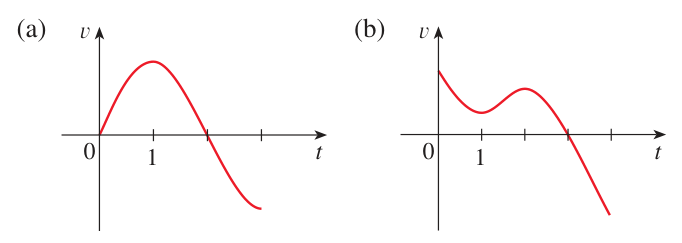
\includegraphics[width=\linewidth]{images/p0270_fig2.png}

    \vspace{7pt}
    \textbf{6.} Đồ thị các hàm \textit{vị trí} của hai chất điểm được cho như hình bên dưới, trong đó $t$ được tính bằng giây. Khi nào vận tốc của mỗi chất điểm mang giá trị dương? Khi nào mang giá trị âm? Khi nào mỗi chất điểm tăng tốc? Khi nào giảm tốc? Giải thích.

    \vspace{3pt}
    \noindent
    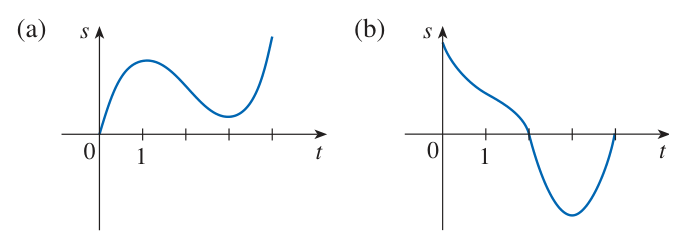
\includegraphics[width=\linewidth]{images/p0270_fig3.png}

    \vspace{7pt}
    \textbf{7.} Giả sử đồ thị hàm vận tốc của một chất điểm được cho như trong hình, trong đó $t$ được tính bằng giây. Khi nào chất điểm chuyển động tiến về phía trước (theo chiều dương)? Khi nào nó chuyển động lùi lại? Điều gì xảy ra khi $5 < t < 7$?
\end{minipage}%
\hfill
\begin{minipage}[t]{0.48\textwidth}
    % CỘT PHẢI (Hình đồ thị & Exercises 8–13)
    \centering
    \vspace*{-3pt}
    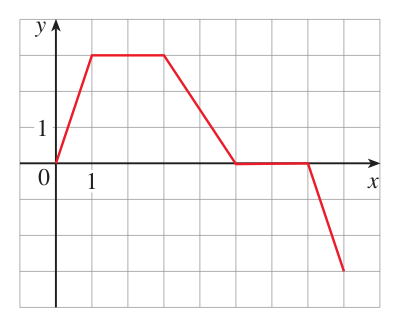
\includegraphics[width=0.62\linewidth]{images/p0270_fig1.png}
    \vspace{4pt}

    \raggedright
    \textbf{8.} Đối với chất điểm được mô tả trong Bài tập 7, hãy phác thảo đồ thị của hàm gia tốc. Khi nào chất điểm tăng tốc? Khi nào giảm tốc? Khi nào nó chuyển động với tốc độ không đổi?

    \vspace{6pt}
    \textbf{9.} Độ cao (tính bằng mét) của một vật thể được bắn thẳng đứng lên trên từ một điểm cách mặt đất $2\text{ m}$ với vận tốc ban đầu $24{,}5\text{ m/s}$ sau $t$ giây là $h = 2 + 24{,}5t - 4{,}9t^2$.
    \begin{enumerate}[label=(\alph*), noitemsep, topsep=1.5pt, leftmargin=16pt]
        \item Tìm vận tốc của vật thể sau $2\text{ s}$ và sau $4\text{ s}$.
        \item Khi nào vật thể đạt độ cao cực đại?
        \item Độ cao cực đại là bao nhiêu?
        \item Khi nào vật thể chạm đất?
        \item Vật chạm đất với vận tốc bằng bao nhiêu?
    \end{enumerate}

    \vspace{5pt}
    \textbf{10.} Nếu một quả bóng được ném thẳng đứng lên trên với vận tốc $80\text{ ft/s}$, thì độ cao của nó sau $t$ giây là $s = 80t - 16t^2$.
    \begin{enumerate}[label=(\alph*), noitemsep, topsep=1.5pt, leftmargin=16pt]
        \item Độ cao cực đại mà quả bóng đạt được là bao nhiêu?
        \item Vận tốc của quả bóng khi nó ở độ cao $96\text{ ft}$ so với mặt đất trong lúc bay lên là bao nhiêu? Trong lúc rơi xuống là bao nhiêu?
    \end{enumerate}

    \vspace{5pt}
    \textbf{11.} Nếu một hòn đá được ném thẳng đứng lên trên từ bề mặt Sao Hỏa với vận tốc $15\text{ m/s}$, độ cao của nó sau $t$ giây là $h = 15t - 1{,}86t^2$.
    \begin{enumerate}[label=(\alph*), noitemsep, topsep=1.5pt, leftmargin=16pt]
        \item Vận tốc của hòn đá sau $2\text{ s}$ là bao nhiêu?
        \item Vận tốc của hòn đá khi nó ở độ cao $25\text{ m}$ trong lúc bay lên là bao nhiêu? Trong lúc rơi xuống là bao nhiêu?
    \end{enumerate}

    \vspace{5pt}
    \textbf{12.} Một chất điểm chuyển động với hàm vị trí
    \[
    s = t^4 - 4t^3 - 20t^2 + 20t \qquad t \ge 0
    \]
    \vspace{-6pt}
    \begin{enumerate}[label=(\alph*), noitemsep, topsep=1.5pt, leftmargin=16pt]
        \item Tại thời điểm nào thì chất điểm có vận tốc bằng $20\text{ m/s}$?
        \item Tại thời điểm nào thì gia tốc bằng $0$? Ý nghĩa của giá trị $t$ này là gì?
    \end{enumerate}

    \vspace{5pt}
    \textbf{13.} (a) Một công ty sản xuất vi mạch máy tính từ các tấm wafer silicon hình vuông. Một kỹ sư quy trình muốn giữ cho độ dài cạnh của tấm wafer rất gần với $15\text{ mm}$ và cần biết diện tích $A(x)$ của tấm wafer thay đổi như thế nào khi độ dài cạnh $x$ thay đổi. Tìm $A'(15)$ và giải thích ý nghĩa của nó trong tình huống này.\par
    \vspace{2pt}
    (b) Chứng minh rằng tốc độ thay đổi diện tích của một hình vuông theo độ dài cạnh bằng một nửa chu vi của nó. Hãy thử giải thích theo quan điểm hình học tại sao điều này đúng bằng cách vẽ một hình vuông có độ dài cạnh $x$ tăng thêm một lượng $\Delta x$. Bạn có thể xấp xỉ độ thay đổi diện tích $\Delta A$ tương ứng như thế nào nếu $\Delta x$ nhỏ?
\end{minipage}
